\documentclass{llncs}
\usepackage{llncsdoc}

\usepackage{graphicx}   
\usepackage{amsmath}

\begin{document}

	\title{SemanticPaint}
	\author{Adam Kosiorek
	\thanks{Advisor: M.Eng.~Keisuke Tateno, Chair for Computer Aided Medical Procedures \& Augmented Reality, TUM, WS 2015/16.}}
	\markboth{Master Seminar: Recent Trends in 3D Computer Vision}{}
	\institute{}
	\maketitle

\begin{abstract}
	The short abstract (50-80 words) is intended to give the reader an overview of the work.
\end{abstract}

\section{Introduction}
  
  Capturing your own environment has never been easier. SemanticPaint can register your surroundings which, after 3D reconstruction, can be semantically segmented in an interactive way. Not only it works in real time but also requires no pretraining. Adding new object categories on the fly is facilitated by online model updates. The user is provided with instantaneous feedback and can re-label any object to correct errors. SemanticPaint makes capturing customized environment models with object classes particular to the user's interest easy and efficient.  
  
  The pipeline starts with capturing the environment as a stream of noisy RGBD images and combining them into a  3D model updated in an online fashion. The user can choose which objects to label and can do so by ``touching'' a small part of an object or encircling it with his hand and uttering the label. The label and the affected data points are further passed to a Streaming Random Forest (SRF) classifier which constantly learns and labels all visible voxels. To further improve classification results a spatially dense labeling is produced by an efficient mean-field inference algorithm. One of the biggest strengths of SemanticPaint is the efficiency of each part of the pipeline, which translates to real time performance. Algorithms used in the pipeline were adapted to work on volumetric data in the TSDF format directly in order to avoiding costly conversions to mesh or point-cloud formats. To allow this, the Voxel Oriented Patch features --- a new type of a discriminative feature describing the voxel space --- has been designed. 
 
\section{Related Work}

  \textbf{Acquisition and Reconstruction } Capturing the geometry of the surrounding world has been a long standing problem \cite{old}. An offline processing of multiple images allowed to reconstruct digital heritage and construct world-scale 3D models with remarkable quality \cite{heritage}. The inception of low-cost RGBD sensors and powerful GPUs enabled online 3D scanning, augmented reality and using 3D environment models for navigation purposes \cite{fusion}. \cite{Monofusion} enables 3D reconstruction of small scenes using a single off-the-shelf RGB camera. It uses a sparse tracking method to first estimate the camera's pose and then select key frames and relative to them secondary frames, from which 3D stereo reconstruction is performed. The achieved results are similar to KinectFusion with the only limitation being that the precision of texture-less surfaces' reconstruction is somewhat lacking. 
  
  \noindent
  \textbf{Scene Understanding } Object recognition, detection and segmentation has been done with 2D RGB images, RGBD data, point clouds and volumetric representations. \cite{VCRF} uses a Voxel-based CRF for simultaneous reconstruction and segmentation. Each voxel contains information about visibility and occlusion as well as group membership. The first two are used to to improve reconstruction by mitigating depth-map noise. The visibility values are constrained by that each ray from the camera can hit only one visible vertex. The group membership information encodes priors given by bounding boxes of detected objects. A graph-cut algorithm is used for global inference. The whole scene has to be registered beforehand, since any change in the CRF's structure would require restarting the inference algorithm. No computational performance was reported. \cite{ChangeDetection} is a first step towards online simultaneous registration and segmentation. Using RGBD images, the framework constructs a model of the environment and updates it each time a new frame comes in. When a significant change in the model is detected, the resulting model is split into a static and a dynamic part, where the latter is assumed to have moved in space. The movement is detected by comparing the expected and observed intensity values at each voxel. The system is online, but is far from real time with 0.7 to 2s processing time per frame. \cite{mesh} shows that converting to another data representation can help to improve segmentation accuracy and inference speed. TSDF model is used to reconstruct a 3D scene from a sequence of RGBD images. The volumetric representation is triangulated and a 3D mesh is recovered. Next, visual features are computed directly on images and projected into the 3D model, while geometric features are computed on the mesh directly. Segmentation is done via a CRF. The approach is tested on the augmented KITTI and NYU datasets for indoor and outdoor scene segmentation where it delivers state-of-the-art results. 
      
  
    
    
% Areas:
%   1. Geometry Acquisition and 3D Reconstruction Techniques:
%     1) digitized cultural heritage with remarkable quality [Levoy et al. 2000]
%   
%     2) world-scale, Internet-accessible, 3D maps reconstructed using street-side [Pollefeys et al. 2008], aerial [Hirschmuller 2008] and online photo collections [Snavely et al.2006; Shan et al. 2013]
% 
%     3) Methods for real-time dense reconstructions, even over large physical scales, with only a single commodity depth or RGB camera have been demonstrated [Rusinkiewicz et al. 2002; Newcombe et al. 2011; Izadi et al. 2011; Newcombe et al. 2011; Chen et al. 2013; Nießner et al. 2013; Pradeep et al. 2013]. Applications such as: live 3D scanning, physically-plausible augmented reality, autonomous robot or vehicle guidance, and 3D fabrication.
%       
%   2. Scene Understanding and Semantic Modeling - interpreting the content of captured 3D models:
%   
%     1) 2D: automatically partition RGB image into semantically meaningful regions [Shotton et al. 2006]
%     
%     2) geometric reasoning to extract 3D structure from single RGB images [Gupta et al. 2010] or exlicit object detection [Yao et al. 2012]).
%     
%     3) RGB + Depth [Silberman and Fergus 2011; Silberman et al. 2012; Couprie et al. 2013; Ren et al. 2012; K ̈ahler and Reid 2013]
%     
%     4) 3D point clouds [Brostow et al.2008; Koppula et al. 2011; Anand et al. 2013; St ̈uckler et al. 2013]
%     
%     5) meshes [Valentin et al. 2013]
%     
%     6) voxel representations [Kim et al. 2013; Karpathy et al. 2013; Salas-Moreno et al. 2013; H ̈ane et al.2013]. 
%       
%     7) semantic segmentation of meshes [Chen et al. 2009]
%     
%     9) dense segmentation of reconstructed scenes [Lin et al. 2013; Sengupta et al. 2013; Ladick`y et al. 2012; Valentin et al. 2013], even in an online manner [Herbstet al. 2014]
%     
%     10) localize objects in small scenes [Abdelrahman et al.2013; Bonde et al. 2013; Karpathy et al. 2013; Lin et al. 2013]
%     
%     11) replace objects with synthetic models [Salas-Moreno et al. 2013; Kim et al. 2012; Shao et al. 2012; Nan et al. 2012; Wang et al. 2014].
%       
%     12) capturing large and compelling datasets which have moved from traditional 2D object images to RGB-D and full 3D scenes [Xiao et al. 2010; Xiao et al. 2013; Geiger et al. 2012].
%     
%     
%   3. Computer Graphics
%   
%     1) automatically segmenting 3D meshes into semantic parts [Chen et al. 2009; Kalogerakis et al. 2010; Shapira et al. 2010; Kim et al. 2013], including incremental depth camera-based methods [Shen et al. 2012]. Most of these methods consider only connected noise-free meshes, and geometric properties, ignoring the appearance. Furthermore, these techniques operate only on single objects, and do not operate in real-time.
%     
%     2) matching scan data to synthetic 3D model databases [Kim et al. 2012; Nan et al. 2012; Shao et al. 2012], with the aim to replace  noisy point clouds with detailed CAD models. These approaches are compelling in that they increase final reconstruction fidelity and exploit repetition of objects to minimize the memory footprint. These systems first perform automatic or interactive segmentation of the scene into constituent parts which are then individually matched to the model database. However, these techniques require a model database to be built and learned offline, and the test-time matching techniques can take seconds to minutes to perform.
%     
%     5) online SLAM system that can recognize objects and update the model live [Salas-Moreno et al. 2013] the model database is still captured and generated offline. Only a single object class (chair) is recognized and it is unclear how the system can support larger surfaces such as floors, walls and ceilings. However, this system demonstrates the power of semantic recognition alongside the reconstruction process, improving relocalization, memory efficiency, and loop closure.
%     
%     6) This type of semantic information has also been explored in the context of bundle adjustment [Fioraio and Di Stefano 2013], and extended to sparse map representations [Ramos et al. 2008; Castle et al. 2007].
%     
%   4. Outdoor Scene Labeling:
%   
%     1) classification of images [Brostow et al. 2008; Posner et al. 2009; Ladick`y et al. 2012]. 
%     
%     2) Dense semantic 3D reconstruction with labeling performed on the images and projectred to the final model, which limits the use of full 3D geometry in their inference [Sengupta et al. 2013].
%     
%     3) Joint volumetric dense reconstruction and semantic segmentation using computationally complex global optimization [H ̈ane et al. 2013].
%     
%     4) Decomposition of outdoor scenes into semantic part; employs 3D model matching techniques similar to [Kim et al. 2012; Nan et al. 2012; Shao et al. 2012] to create reconstructions from LiDAR data [Lin et al. 2013]. None of these systems operate in a real-time or in an online manner.    
%     
%   5. Indoor Scene Recognition:
%   
%     1) using RGB-D sensors [Silberman and Fergus 2011; Silberman et al. 2012; Couprie et al. 2013; Ren et al. 2012; K ̈ahler and Reid 2013]. Classification or recognition is performed in image-space, along with 3D priors to aid segmentation. Again these systems fail to exploit full 3D geometry and are the counterpart of image-based segmentation but for RGB-D frames. 
%     
%     2) [Valentin et al. 2013] exploits 3D meshes and geometric and appearance features for improved inference in outdoor and indoor scenes.
%     
%     3) [Kim et al. 2013] use a voxel-based conditional random field (CRF) for segmentation and occupancy-grid based reconstruction.
%     
%     However, these techniques are not efficient enough to be used in an online system, and operate only on coarse reconstructions.
%     
%     
% Our approach differs from these systems in several compelling
% ways. Firstly our system runs entirely online and interactively, in-
% cluding data capture, feature computation, labeling, segmentation,
% learning and filtering. Second, our pipeline leads to robust and dense
% object labels directly on the acquired 3D model. Finally, in our
% system, the user is ‘in the loop’ during the labeling and training
% process, allowing the system to evolve to new object classes in an
% online fashion, and allowing the user to label a minimal amount and
% correct any mistakes interactively. This allows the user to rapidly
% build up models personalized to their spaces and goals
   


\section{Space Representation}
   
  The space is represented by a 3D volume constructed from the sequence of RGBD images using Truncated Signed Distance Function (TSDF) \cite{TSDF}. Large-scale scene handling is facilitated by the hashed volumetric representation of \cite{hashed_voxel} with a 6mm$^{3}$ voxel. Each voxel contains: TSDF distance, colour information in the LAB space, a weight for averaging distance values, a user annotation class, a predicted class, an outcome of the mean-field inference from before and after classification and the probability of each class as inferred by the mean-field algorithm, for each class. The total number of bits per voxel is $96 + \textrm{[number of classes]} \cdot 16$.

\section{Voxel Oriented Patches}

\begin{figure}
 \center
 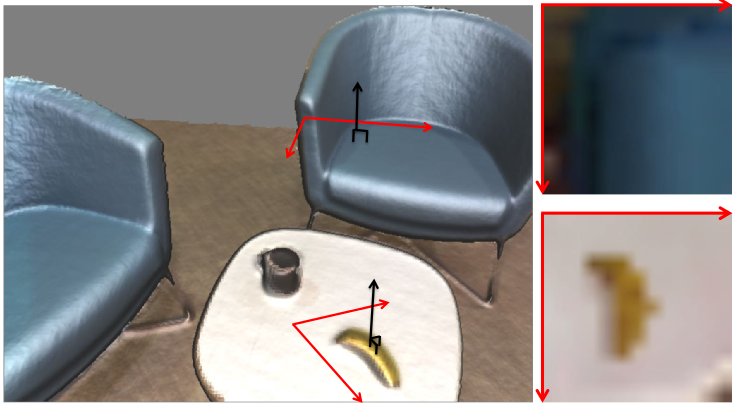
\includegraphics[width=0.75\textwidth]{figures/vop}
 \caption{Voxel Oriented Patch. Colours shown in RGB for illustration purposes.}
 \label{fig:vop}
\end{figure}

  This work relies heavily on classification and since even the most powerful classifier is useless if inappropriate features are supplied this paper contributes Voxel Oriented Patch (VOP) features. They are efficiently computed from the TSDF volume representation (cf. figure \ref{fig:vop}). Let $V_i$ be a VOP and $\mathbf{n}^i$ the normal of voxel i. An image patch of dimensions $r \times r$  is centered on voxel $i$ from the plane $(\mathbf{p} - \mathbf{p}_i) \cdot \mathbf(n)_i = 0$. The patch contains colour values stored in the TSDF on the plane in CIELab to mitigate illumination effects. Additionally, $V_i$ stores distance to the nearest dominant horizontal surface. $r = 13$ with a resolution of $10\frac{mm}{pixel}$ is used. Rotation invariance is achieved exactly as in \cite{sift}. The patch is rotated according to the dominant gradient direction. It is computed by creating a histogram of gradient directions with 36 bins, where the directions are weighted by gradient magnitudes and a gaussian window centered at the voxel. Furthermore, a quadratic polynomial is fit to the three biggest values of the histogram, whose maximum is the final direction. 

\section{Streaming Random Forests}
  
  A random forest is an ensemble of classification or regression trees, whose outputs are combined to produce a result with lower variance \cite{online_forest}. Each tree is typically trained only on a subset of the training data $S$ comprised of pairs $(i, l)$ where $i$ is a sample and $l$ its label.  Let $f(i; \theta) \in \{L, R\}$ denote the binary split function with learned parameters $\theta$, which specify a feature this node uses. The tree's output amounts to the probability distribution $P_F(x_i = l | \mathbf{D})$ stored at each node. Trees learn in a greedy way: for each node a split function is chosen from a distribution $\Theta$ of candidate split functions to maximize the information gain. 
  
  \begin{equation} \label{eq:infogain}
   G(S, S^L, S^R) = H(S) - \sum_{d \in \{L, R\}} \frac{|S^d|}{|S|}H(S^d)
  \end{equation}
  
  Where $H(S) = - \sum_{(l, i) \in S} p(c_i = l) \log{p(c_i = l)}$ is Shannon Entropy. Training set is then split into subsets $S^d(\theta)$, $d \in \{L, R\}$ used to train child nodes. This procedure requires that all training data is available.
  
  Online Random Forest \cite{online_forest} allow runtime model updates and they differ in that for a new node $n$ they generate a distribution of split function $\Theta_n$ and maintain a set of label statistics for each of them, updated when a new sample comes to the node. Label statistics are sufficient to compute information gain and thus the node $n$ is further split if it has seen a predefined number of samples or if the minimal value of the information gain is low enough. Storing and updating statistics in leaf nodes is computationally expensive which limits runtime performance
  
\begin{figure}[!ht]
  \center
  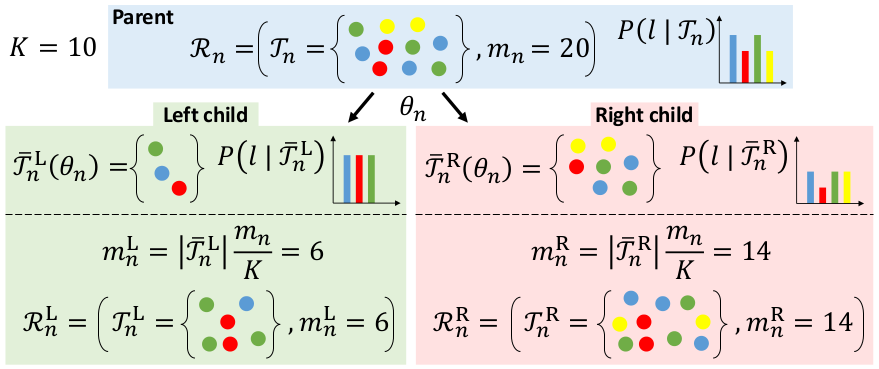
\includegraphics[width=0.75\textwidth]{figures/forest}
  \caption{Splitting reservoirs in Streaming Random Forest.}
  \label{fig:forest}
\end{figure}
  
  Streaming Random Forest begins by creating a reservoir $R_n$ of at most $K$ samples stored in a list $T_n$ at the root node. It represents an unbiased sample of all training data seen so far. Initially, the first $K$ samples are stored. Then, a sample in the reservoir is exchanged with an incoming one with probability $p = \frac{K}{m_n}$, where $m_n$ is the number of samples seen so far at node $n$. Splitting the node requires computing the objective function for each $\theta \in \Theta_n$ over $R_n$. $H(R_n)$ is computed from the normalized class label histogram $P(l|R_n)$. Let $|R_n|$ be the amount of samples stored in the reservoir $n$ and let $R_n^d$ be the splitting induced by $\theta$. Finally, the split function is chosen as $f_n = \arg \max_{\theta \in \Theta_n} G(S, S^L, S^R | \theta)$  and set the number of samples seen by the child node to $|m_n^d| = |R_n^d| \max {\left(1, \frac{m_n}{K}\right)}$. Since the total number of samples stored is bounded by $K$ this approach uses less memory. Constructing child reservoirs from parent reservoirs (cf. fig \ref{fig:forest}) lessens the computational load.
  
  The GPU implementation can handle up to 17 million voxel classifications per second, while between 3 and 10 million voxels are visible at any one time \cite{hashed_voxel}. To improve performance, voxels are batched and only a single batch is evaluated per frame.

\section{Dynamic Conditional Random Field}

 Conditional Random Fields are often used for segmentation \cite{VCRF}, but they usually assume availability of all data. Here, a pairwise CRF \cite{crf} with a time dependent underlying model is used. It requires a novel inference algorithm that can handle updates of the geometry and user specified labels. The class of each voxel is modeled by a random variable $x_i$. The label distribution over the volume $\mathcal{V}$ factorizes into likelihood terms $\psi_i(x_i)$ and prior terms $\psi_{ij}(x_i, x_j)$. Let $\mathcal{E}_i$ be a neighbourhood of $v_i$, $\mathbf{D}_t $ volumetric data at time $t$ and $\mathbf{x}$ a vector of all $x_i$. The posterior distribution is given by
 
  \begin{equation} \label{eq:posterior}
  P(\mathbf{x}|\mathbf{D}) = \prod_{i \in \mathcal{V}} \left( \psi_i(x_i) \prod_{j \in \mathcal{E}_i} \psi_{ij}(x_i, x_j) \right) 
  \end{equation}

  Neighbourhood of 6 cm is used. Negative log likelihood of eq. \ref{eq:posterior} defines the energy

  \begin{equation} \label{eq:energy}
  E_t(\mathbf{x}) = \sum_{i \in \mathcal{V}} \left( \phi_i(x_i) + \sum_{j \in \mathcal{E}_i} \phi_{ij} (x_i, x_j) \right) + K
  \end{equation}

  Unary and pairwise potentials $\phi_i(x_i)$ and $\phi_{ij}(x_i, x_j)$ encode the cost of assigning a label to $v_i$ and a cost of assuming different labels by voxels in a neighbourhood, respectively. These costs are constantly changing due to the changing predictions of the random forest and user interaction. 

  Initially, all voxels are encouraged to take a background label by setting $\phi_i(l) = 0$ for background class and grater than zero otherwise. When the user touches an object, a set of touched voxels $\mathcal{H}_S$ is registered and their unary potentials set to $\phi_i(l) = \infty$ if their labels are different then the specified one, and zero if they are the same, thus imposing the labeling. If user labels a region more than once, the old labels are simply overwritten. 
   
  To process the encircling action, the labeling is projected into the current frame. Next, a GMM is fit with the foreground class taken as a convex hull of the encircled region and background as the rest of the image. For every pixel in a bounding box around the user annotation the unary potentials are updated as 

  \begin{equation}
  \phi_i(l) =
    \begin{cases}
      \log P_E(fg|\mathbf{a}_i)       & \quad \text{if } l = \text{fg}\\
      \log (1 - P_E(fg|\mathbf{a}_i))  & \quad \text{if } l = \text{bg}\\
    \end{cases}
  \end{equation}

  with $P_E($fg$|\mathbf{a}_i)$ the probability of assuming the foreground label, which stems from the normalized likelihood $P(\mathbf{a}_i|$fg$)$ from the GMM.

  \begin{equation}
    P_E(\text{fg}|\mathbf{a}_i) = \frac{P(\mathbf{a}_i|\text{fg}) }{P(\mathbf{a}_i|\text{fg}) + P(\mathbf{a}_i|\text{bg})}
  \end{equation}

  For all voxels that haven't been explicitly labeled by the user unitary potentials are updated with the predicted values as $\phi_i(l) = -\log P_F(x_i = l | \mathbf{D})$. Finally, smoothness is achieved by the standard Potts model by assigning a discontinuity cost $\phi_{ij}(x_i, x_j) = \lambda_{ij}$ if voxels have different labels and zero otherwise, with $\lambda_{ij}$ a function of difference in position, intensity and normal directions.

\section{Efficient Mean-Field Inference}

The mean-field inference algorithm is adapted from \cite{inference} to handle the constantly changing energy landscape and implemented on GPU. First, the original probability distribution $P(\mathbf{x})$ is approximated by $Q(\mathbf{x})$ under KL-divergence $KL(Q||P)$.  $Q(\mathbf{x})$ is chosen such that the marginal of each random variable is independent, that is $Q(\mathbf{x}) = \prod_i Q_i(\mathbf{x)_i})$. Iterative updates yield:

\begin{equation}
 Q_i^t(l) = \frac{1}{Z_i}e^{M_i(l)} \text{, } t = 1, \ldots, T
\end{equation}
\begin{equation}
 M_i(l) = \phi_i(l) + \sum_{l' \in \mathcal{L}} \sum_{j \in \mathcal{N}(i)} Q_j^{t-1}(l')\phi_{ij}(l, l')
\end{equation}

with $Z_i$ a normalizing factor and final class chosen as the minimizer of $Q_i^T$. Energy distribution is assumed to change only gradually. Moreover, SRF classification results would impact the final segmentation after several frames due to their effect on unitary potentials. To speed up the process the initial energy value at a new frame is set to a weighted sum of the previous frame's state and the SRF prediction. It works well in practice and allows visually pleasing label propagation effect.

\begin{equation}
 \widetilde{Q}_i^t(x_i) = \gamma Q_i^{t-1}(x_i) + (1 - \gamma) P_F^{t-1}(x_i = l | \mathbf{D}) \text{, } \gamma \in [0, 1]
\end{equation}

% \section{Putting it All Together}
% 
%   The user comes into a room and touches a table uttering a label at the same time. Then, he touches a chair giving another label. He switches into test mode and goes into another room. All tables and chair are marked by the system accordingly. It works by feeding Voxel Oriented Patches associated with each pixel to the Streaming Random Forest, which learn to predict voxel categories in an online fashion. User interactions are facilitated by a Conditial Random Field that models the label distribution. An efficient mean-field algorithm, which amortizes classification of the whole scene among several frames, is used on top of it to smooth predicted labels.

\section{Results}
  Each part of the pipeline is evaluated separately. Several video sequences were recorded to evaluate segmentation and VOP features. A set of key frames covering the whole scene from each sequence was hand-labeled to create groundtruth data. They were further projected into the 3D volume, resulting in 4176, 12346, 7583, 8916 frames for \emph{LivingRoom}, \emph{Kitchen}, \emph{Bedroom} and \emph{Desk} sequences respectively, of which around a third was used for testing. Table \ref{fig:segm_results} summarizes segmentation results. User interaction gives very accurate labeling, but it affects a single object instance only. SRF prediction works well and is improved by further inference. Table \ref{fig:vop_results} compares VOPs against other features. The numbers reflect the percentage of correctly classified pixels with SRF using different features. VOP clearly outperforms all other features. $\Delta$ RGB mean stands for the mean difference of two randomly selected patches. 
  
  
\begin{table}[!ht]	
 \center
 \caption{Segmentation Results.}
 \begin{tabular}{c|c|c|c|c|c}
  \textbf{Component} & \textbf{LivingRoom} & \textbf{Bedroom} & \textbf{Kitchen} & \textbf{Desk} & \textbf{Average} \\ \hline
  User Interaction & 99.35\% & 97.61\% & 96.09\% & 97.73\% & 97.7\% \\ 
  Forest Prediction & 94.57\% & 88.31\% & 82.58\% & 90.29\% & 88.94\% \\
  Final Inference & 96.26\% & 95.19\% & 90.69\% & 95.55\% & 94.42\%
 \end{tabular}
 \label{fig:segm_results}
\end{table}


\begin{table}[!ht]	
 \center
 \caption{Comparison of VOP against other features.}
 \begin{tabular}{c|c|c|c|c|c}
  \textbf{Feature} & \textbf{LivingRoom} & \textbf{Bedroom} & \textbf{Kitchen} & \textbf{Desk} & \textbf{Average} \\ \hline
  VOP & \textbf{94.57\%} & \textbf{88.31\%} & 82.58\% & \textbf{90.29\%} & \textbf{88.94\%} \\
  $\Delta$ RGB mean & 80\% & 71.84\% & 76.29\% & 73.42\% & 75.39\% \\
  Depth probe& 77.54\% & 61.79\% & \textbf{84.9\%} & 68.9\% & 73.06\% \\
  Color Probe& 56.39\% & 65.68\% & 60.77\% & 60.74\% & 60.9\% \\
  SURF & 43.74\% & 67.12\% & 57\% & 58.13\% & 56.5\% \\
  SPIN & 58.77\% & 43.22\% & 48.41\% & 36.1\% & 46.63\% \\
 \end{tabular}
 \label{fig:vop_results}
\end{table}

  SRF was compared against Online Random Forests (ORF) \cite{online_forest} and Hoeffding trees (HT) \cite{htree}. In order to simulate non-IID data, a dataset of 300 objects of 51 categories \cite{dataset} was used. One revolution of each object was recorded with an RGBD camera from three different viewpoints. Online setting was created by sequentially adding new categories. Two thirds of each viewpoint of each object is used for training. Results are summarized by figure \ref{fig:srf_results}. SRF clearly outperforms its competitors.

\begin{figure}[!ht]
 \center
 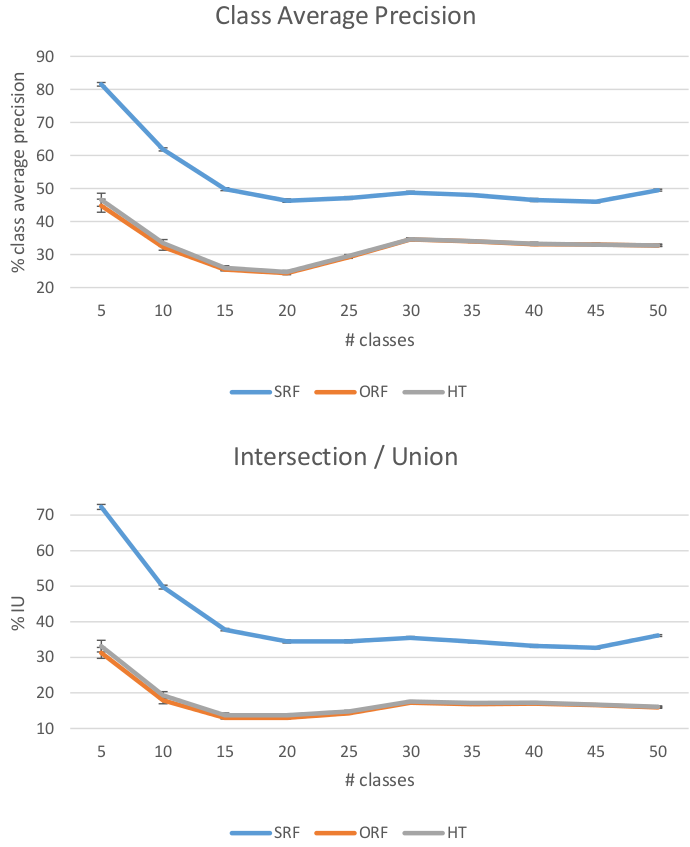
\includegraphics[width=0.75\textwidth]{figures/srf_results}
 \caption{Comparison of Streaming Random Forest against Online Random Forest and Hoeffding Trees.}
 \label{fig:srf_results}
\end{figure}

\section{Discussion}

  This paper contributes an interactive system that enables users to create customized models of 3D environments. It can be used to gather groundtruth for large-scale visual recognition systems, robot navigation and to aid partially sighted people. There are some limitations, however. Use of the system is now restricted to simple indoor scenes. Computational load increases with the size of the scene while prediction accuracy drops with the number of object categories.
  
\begin{figure}[!ht]	 
 \center
 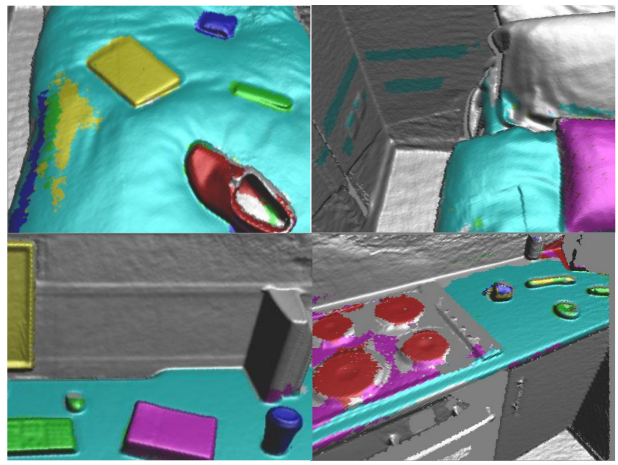
\includegraphics[width=0.75\textwidth]{figures/failures}
 \caption{Failure cases.}
 \label{fig:failures}
\end{figure}
  
  The system has also some limitations. Combing colour and depth data requires careful sensor calibration. Combing colour and depth data requires careful sensor calibration. Lack thereof results in misclassification at object boundaries. Additionally, strong changes of lighting conditions impair classification ability at certain viewpoints. These failures are shown in figure \ref{fig:failures}. Moreover, computational performance drops with the increasing size of the scene and classification accuracy decreases with the number of classes. What is more, no global context is used for classification. 

\section{Future Work}
  
  There is big room for improvement. Introducing priors associated with the type of environment or with an object class (\emph{e.g.} vertical walls) could greatly improve classification accuracy. Failure cases from Fig. \ref{fig:failures} could be avoided if pure geometric features were used. Some research is required on scaling the system to bigger scenes and moving to outdoor environments. 

\bibliographystyle{splncs}
\begin{thebibliography}{1}

  \bibitem{old}
  ROBERTS , L. G. 1963. Machine perception of three-dimensional solids. Ph.D. thesis, Massachusetts Institute of Technology.

  \bibitem{VCRF}
  KIM , B.-S., KOHLI , P., AND SAVARESE , S. 2013. 3D scene understanding by voxel-CRF. In Proc. ICCV.

  \bibitem{Monofusion}
  PRADEEP , V., RHEMANN , C., IZADI , S., ZACH , C., BLEYER , M., AND BATHICHE , S. 2013. Monofusion: Real-time 3D reconstruction of small scenes with a single web camera. In Proc. ISMAR.

  \bibitem{ChangeDetection}
  HERBST , E., HENRY , P., AND FOX , D. 2014. Toward online 3-d object segmentation and mapping. In IEEE International Conference on Robotics and Automation (ICRA).

  \bibitem{mesh}
  VALENTIN , J. P., SENGUPTA , S., WARRELL , J., SHAHROKNI , A., AND TORR , P. H. 2013. Mesh based semantic modelling for indoor and outdoor scenes. In Proc. CVPR.

  \bibitem{heritage}
  LEVOY , M., PULLI , K., CURLESS , B., RUSINKIEWICZ , S., KOLLER , D., EREIRA , L., GINZTON , M., ANDERSON , S., DAVIS , J., G NSBERG , J., ET AL . 2000. The digital Michelangelo project: 3D scanning of large statues. In Proc. SIGGRAPH. ACM.

  \bibitem{fusion}
  NEWCOMBE , R. A., IZADI , S., HILLIGES , O., MOLYNEAUX , D., KIM , D., DAVISON , A. J., KOHLI , P., SHOTTON , J., HODGES , S., AND FITZGIB-BON , A. 2011. KinectFusion: Real-time dense surface mapping and tracking. In Proc. ISMAR.
  
  \bibitem{TSDF}
  CURLESS , B. AND LEVOY , M. 1996. A volumetric method for building complex models from range images. In Proceedings of the 23rd annual conference on Computer graphics and interactive techniques. ACM, 303–312.
  
  \bibitem{hashed_voxel}
  NIESSNER , M., ZOLLHOFER , M., IZADI , S., AND STAMMINGER , M. 2013. Real-time 3D reconstruction at scale using voxel hashing. ACM TOG 32, 6
  
  \bibitem{online_forest}
  SAFFARI , A., LEISTNER , C., SANTNER , J., GODEC , M., AND BISCHOF , H. 2009. On-line random forests. In IEEE ICCV Workshop.
  
  \bibitem{reservoir}
  VITTER , J. S. 1985. Random sampling with a reservoir. ACM TOMS 11, 1.
  
  \bibitem{sift}
  LOWE , D. G. 1999. Object recognition from local scale-invariant features. In Proc. ICCV.
  
  \bibitem{crf}
  LAFFERTY , J., McCALLUM , A., AND PEREIRA , F. C. 2001. Conditional random fields: Probabilistic models for segmenting and labeling sequence data.
  
  \bibitem{inference}
  KRAHENBÜHL, P. AND KOLTUN , V. 2011. Efficient inference in fully connected CRFs with Gaussian edge potentials. In NIPS.

  \bibitem{kl}
  KOLLER , D. AND FRIEDMAN , N. 2009. Probabilistic Graphical Models: Principles and Techniques. MIT Press
  
  \bibitem{htree}
  DOMINGOS , P. AND HULTEN , G. 2000. Mining high-speed data streams. In Proc. SIGKDD.
	
  \bibitem{dataset}
  LAI , K., BO , L., REN , X., , AND FOX , D. 2011. A large-scale hierarchical multi-view rgb-d object dataset. In Proc. ICRA.


\end{thebibliography}
\end{document}
